\documentclass[../main.tex]{subfiles}
\begin{document}

\appendix
\begin{appendices}

\section{8-spin Problems}
Here, we show some of the important results for the set of 8-spin problems, each consisting of 8 Boolean variables and 9 clauses. Analogous to Fig.~(\ref{fig:f10}), Fig.~(\ref{fig:ap1}) shows the scatter plot of the minimum energy gaps after adding the ferromagnetic trigger against the original minimum energy gaps, for all the 8-spin problems. As in the case of the 12-spin problems, all the minimum energy gaps are enlarged as a result of adding the ferromagnetic trigger, for all the three strengths of the trigger. Moreover, the enlargement is directly proportional to the strength of the trigger.

\begin{figure}[H]
\centering 
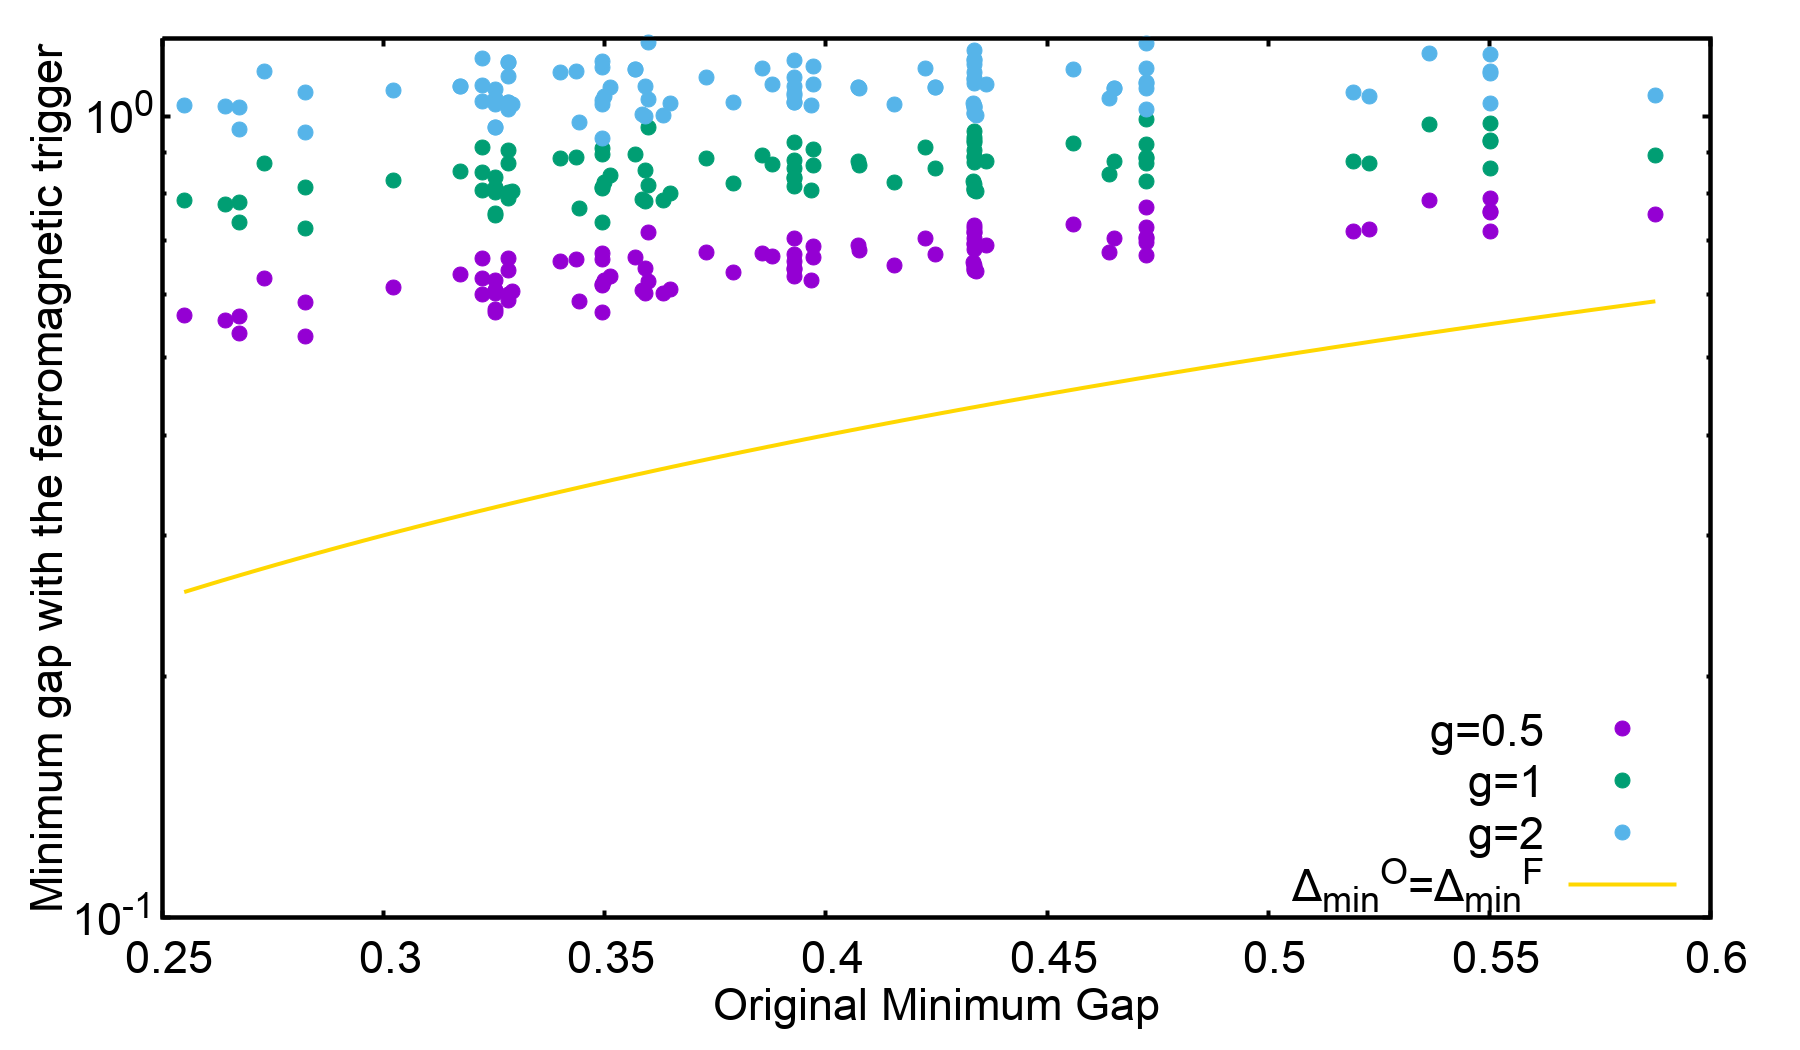
\includegraphics[scale=0.2]{Mingap_F_8.png}
\caption{Scatter plot of the minimum gaps upon adding the ferromagnetic trigger with $g\in$ \{0.5,1,2\} against the original minimum energy gaps. The points lying above the solid line represent the problems with an enlarged minimum gap.}
\label{fig:ap1}
\end{figure}

The corresponding plot with the antiferromagnetic trigger is shown in Figure~(\ref{fig:ap2}).

\begin{figure}[H]
\centering 
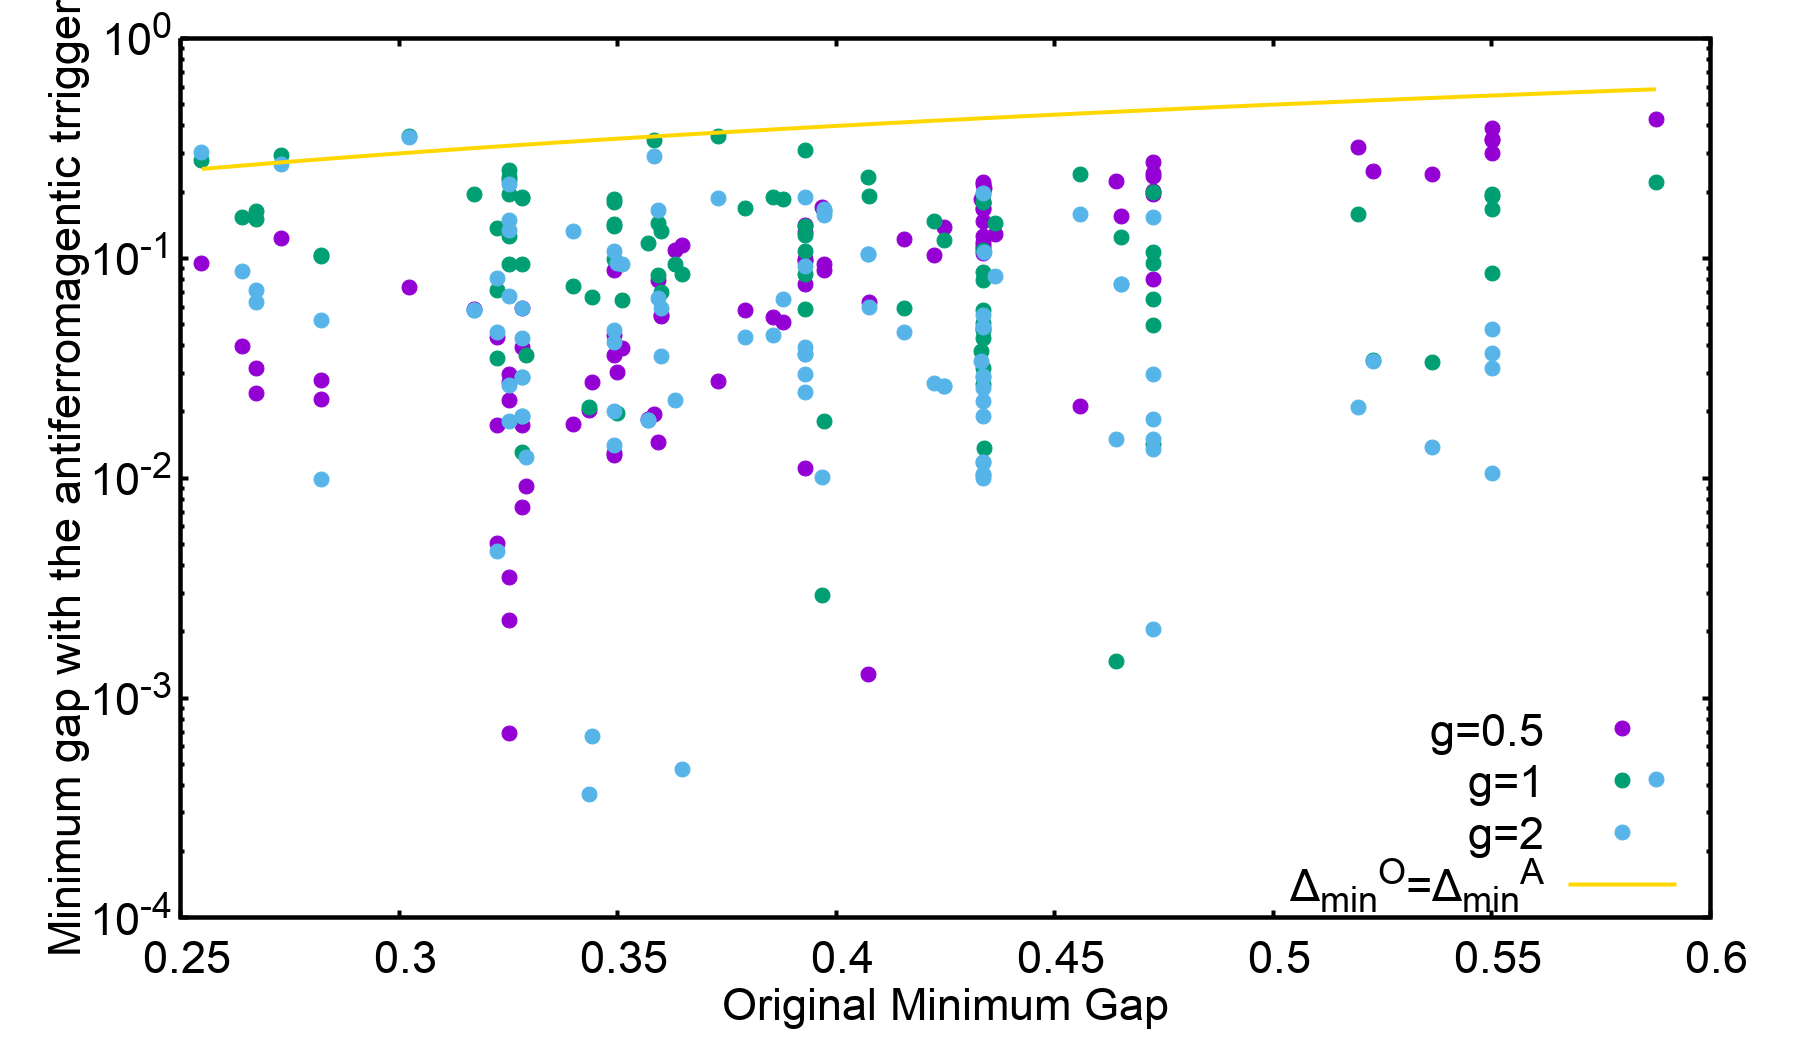
\includegraphics[scale=0.2]{Mingap_A_8.png}
\caption{Scatter plot of the minimum gaps upon adding the antiferromagnetic trigger with $g$ $\in$ \{0.5,1,2\} against the original minimum energy gaps. The points lying above the solid line represent the problems with an enlarged minimum gap.}
\label{fig:ap2}
\end{figure}
The minimum energy gaps after adding the antiferromagnetic trigger are reduced for almost all the cases. For $g$=1 and $g$=2 only two problems have a larger minimum gap after adding the trigger, while for $g$=0.5, all the minimum gaps are reduced.

To obtain an estimate of how adding the ferromagnetic trigger affects the success probability of the 8-spin problems, and the range of the affected problems, a scatter plot of the success probability against the original success probability is given in Figure~(\ref{fig:ap3}). It can be noted that the original success probability in this case, for annealing times of 100 and 1000, is very close to 1, for all the the problems of the set. For this reason the results for only $T_A$=10 have been shown here.

\begin{figure}[H]
\centering 
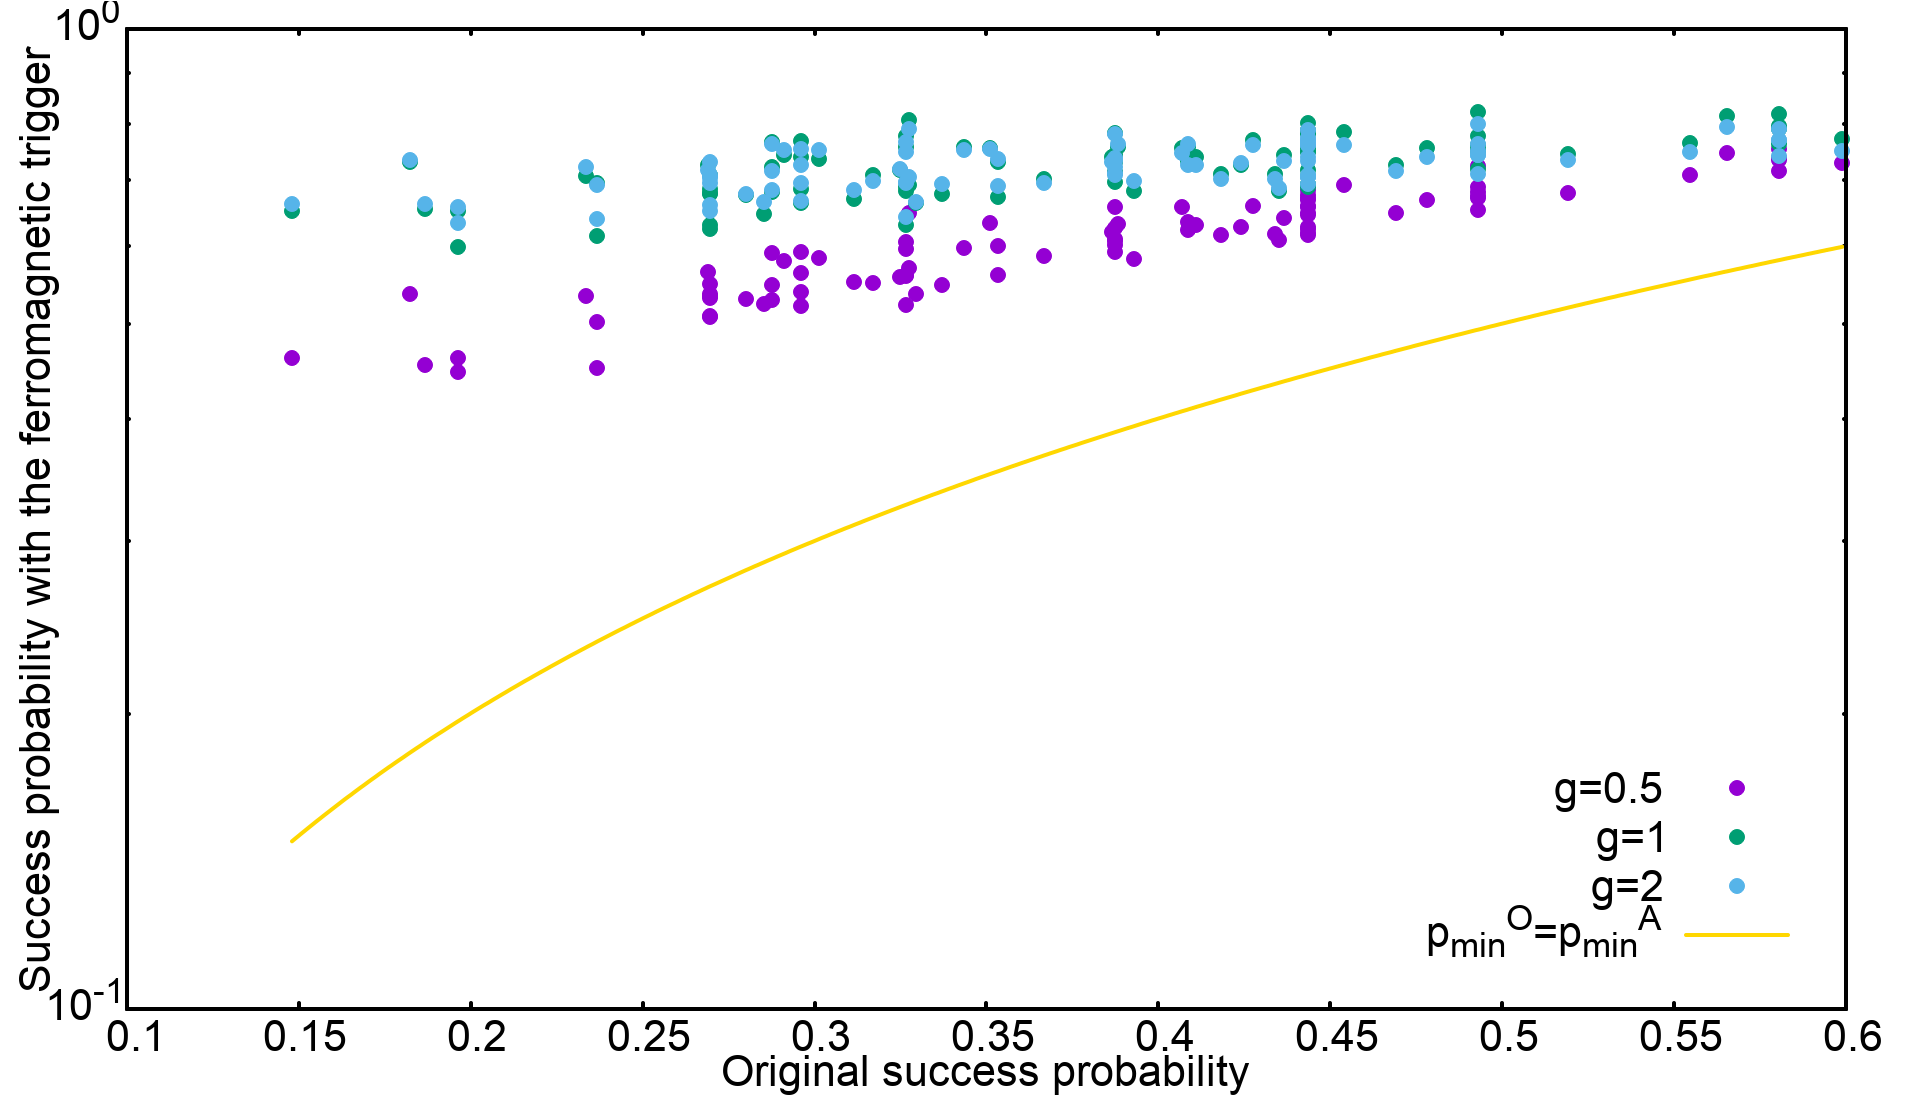
\includegraphics[scale=0.24]{Succ_OF_8.png}
\caption{Scatter plot for the success probability after adding ferromagnetic trigger against the success probability of the original Hamiltonian, for $T_A$=10, with different strengths. The points lying above the solid line represent the problems with an improved success probability.}
\label{fig:ap3}
\end{figure}
From Figure~(\ref{fig:ap3}) it can be observed that the success probability after adding the ferromagnetic trigger is larger than the original success probability for all the problems. Additionally, on increasing the strength of the trigger, the success probability for a certain problem becomes systematically larger. However, on adding the antiferromagnetic trigger the success probabilities decrease for a majority of the cases (see Figure~(\ref{fig:ap4})). Only 3 problems corresponding to $g$=0.5 and $g$=2, and 12 to $g$=1 have a larger success probability after adding the antiferromagnetic trigger. 


\begin{figure}[H]
\centering 
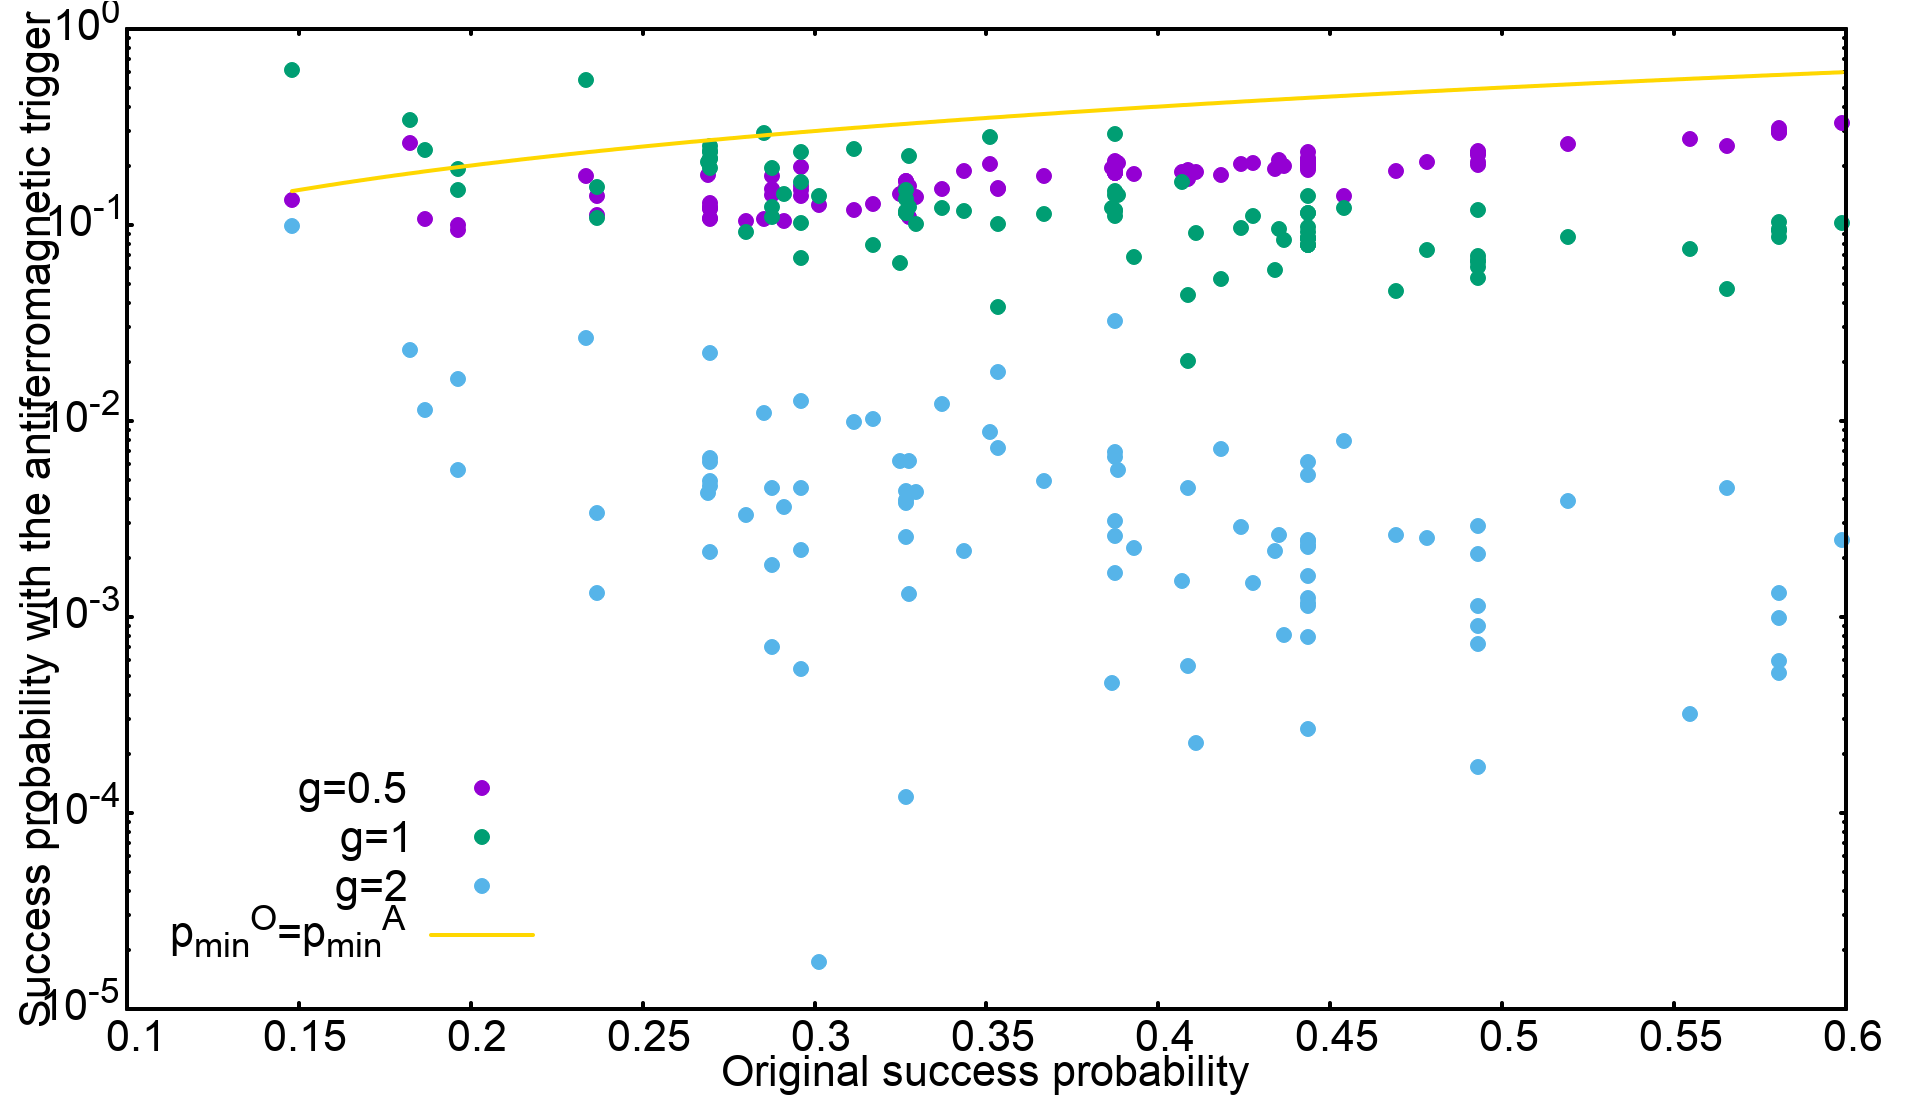
\includegraphics[scale=0.24]{Succ_OA_8.png}
\caption{Scatter plot for the success probability after adding antiferromagnetic trigger against the success probability of the original Hamiltonian, for annealing time $T_A$=10, with different strengths. The points lying above the solid line represent the problems with an improved success probability.}
\label{fig:ap4}
\end{figure}

Finally, a plot of the success probabilities with the minimum energy gaps has been shown before and after adding the triggers, in Figure~(\ref{fig:ap5}).


\begin{figure}
\centering 
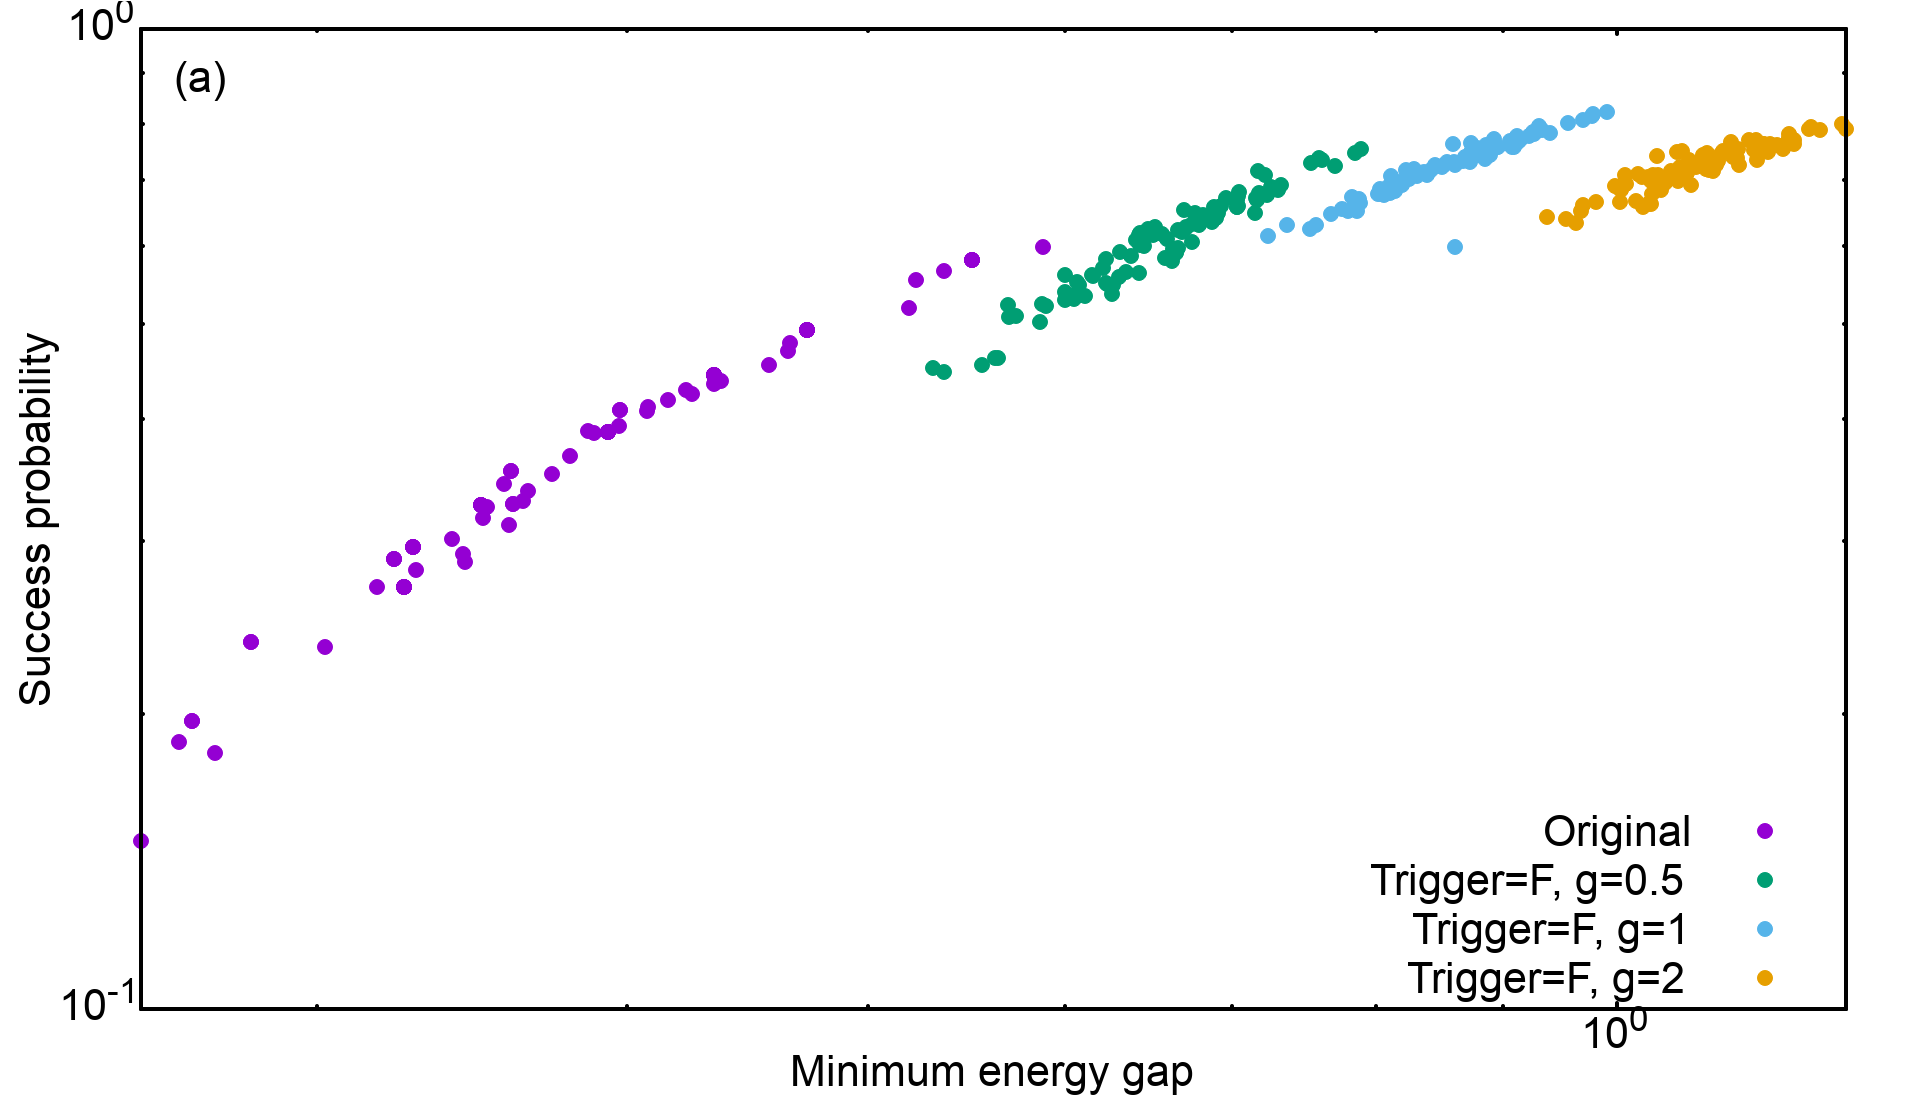
\includegraphics[scale=0.24]{SuccVsGap_F_8.png}
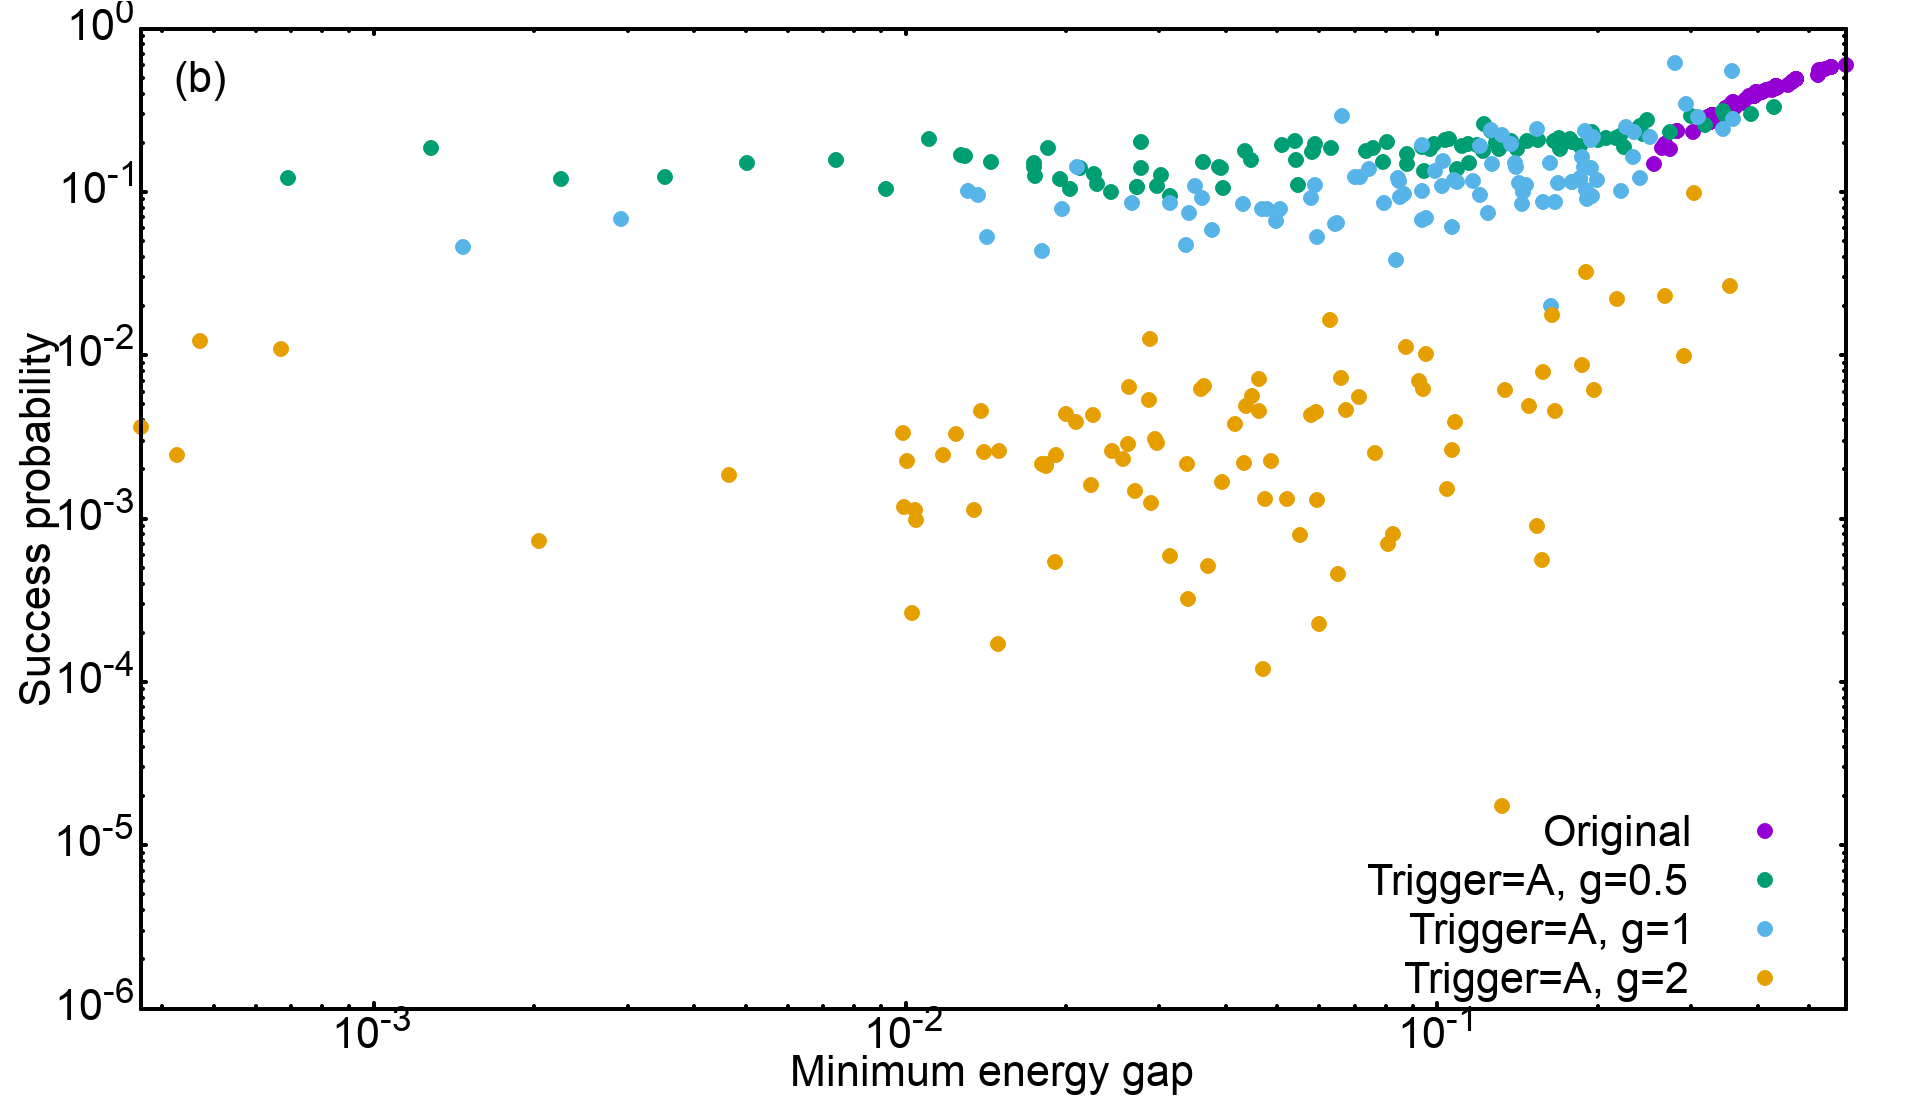
\includegraphics[scale=0.24]{SuccVsGap_A_8.png}
\caption{Plot of the success probability versus minimum energy gaps for all the problems belonging to the set for $T_A$=10. (a): After adding the ferromagnetic trigger; (b): After adding the antiferromagnetic trigger }
\label{fig:ap5}
\end{figure}
The effects of adding the ferromagnetic trigger are very systematic compared to the effects of adding the antiferromagnetic trigger. The minimum gaps become larger with increasing the strength of the trigger, and the success probabilities improve with increasing the annealing time. On the other hand, the overall effect of adding the antiferromagnetic trigger was a significant increase in the scattering of the curves. This trend can be explained on the basis of non-adiabatic mechanisms affecting the success probability for a larger number of problems, since adding the antiferromagnetic trigger reduces the minimum energy gaps for a majority of the problems.

\section{Modelling the energy levels using effective Hamiltonian approach}
For modelling the energy levels after adding the triggers to the original Ising Hamiltonian, the trigger Hamiltonian is regarded as a perturbation to the original Ising Hamiltonian consisting of the initial and the final Hamiltonians, so that 
\begin{equation}
H(t)=H_0(t)+H_T(t),.
\end{equation}
where $H_0$ is the original Hamiltonian, and $H_T$ is the trigger Hamiltonian.\\
For this, we will restrict to the first order perturbation theory, and to the lowest lying energy levels of the original Hamiltonian ($\ket{\psi_0}$ with energy $E_0$ and $\ket{\psi_1}$ with energy $E_1$. Then,
\begin{equation}
a_0'=\bra{\psi_0}H\ket{\psi_0}=E_0+\bra{\psi_0}H_T \ket{\psi_0}=E_0+a_0,
\end{equation}
\begin{equation}
a_1'=\bra{\psi_1}H\ket{\psi_1}=E_1+\bra{\psi_1}H_T \ket{\psi_1}=E_0+a_1,
\end{equation}
\begin{equation}
\bra{\psi_0}H(t)\ket{\psi_1}=\bra{\psi_0}H_T \ket{\psi_1}=a_2,
\end{equation}
with $a_0'$ and $a_1'$ being the diagonal elements of the effective Hamiltonian. The effective Hamiltonian then becomes
\begin{center}
$ H= \begin{pmatrix}
a_0' & a_2\\
a_2* & a_1'
\end{pmatrix}$
\end{center}
If $\Delta_{min}$ is the minimum energy gap between the ground state and the first excited state of the original Hamiltonian, the minimum energy gap between the ground state and the first excited state of the effective Hamiltonian, $\Delta_{min}'$ is thus given as
\begin{equation}
\Delta_{min}'=\sqrt{{(\Delta+a_1-a_0)}^2+4{a_2}^2}.
\end{equation}
However, in order for the approximation to be valid, the value of the strength parameter, $g$, should be small. Thus choosing $g$ to be 0.1, Figure~(\ref{fig:ap8}) shows the modelled energy levels for the effective Hamiltonian, for the ferromagnetic and antiferromagnetic triggers.
\begin{figure}
\centering 
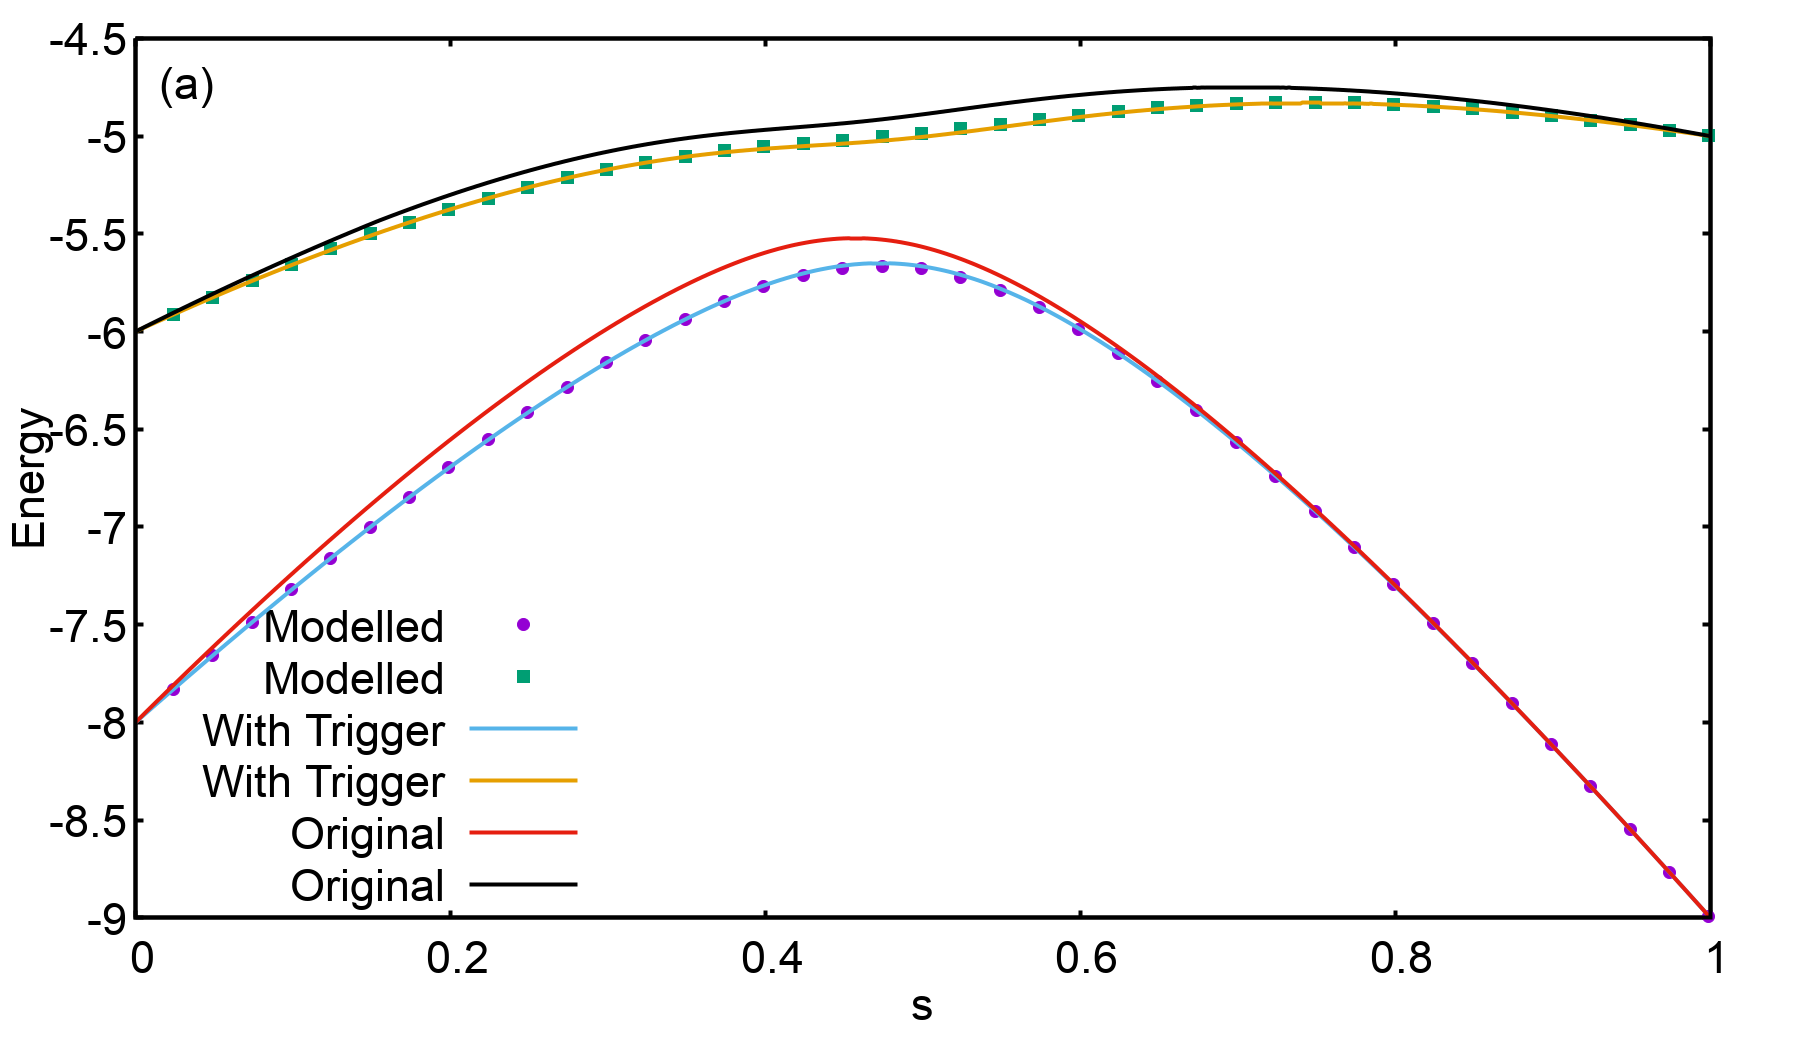
\includegraphics[scale=0.2]{98_Ferro_g0.png}
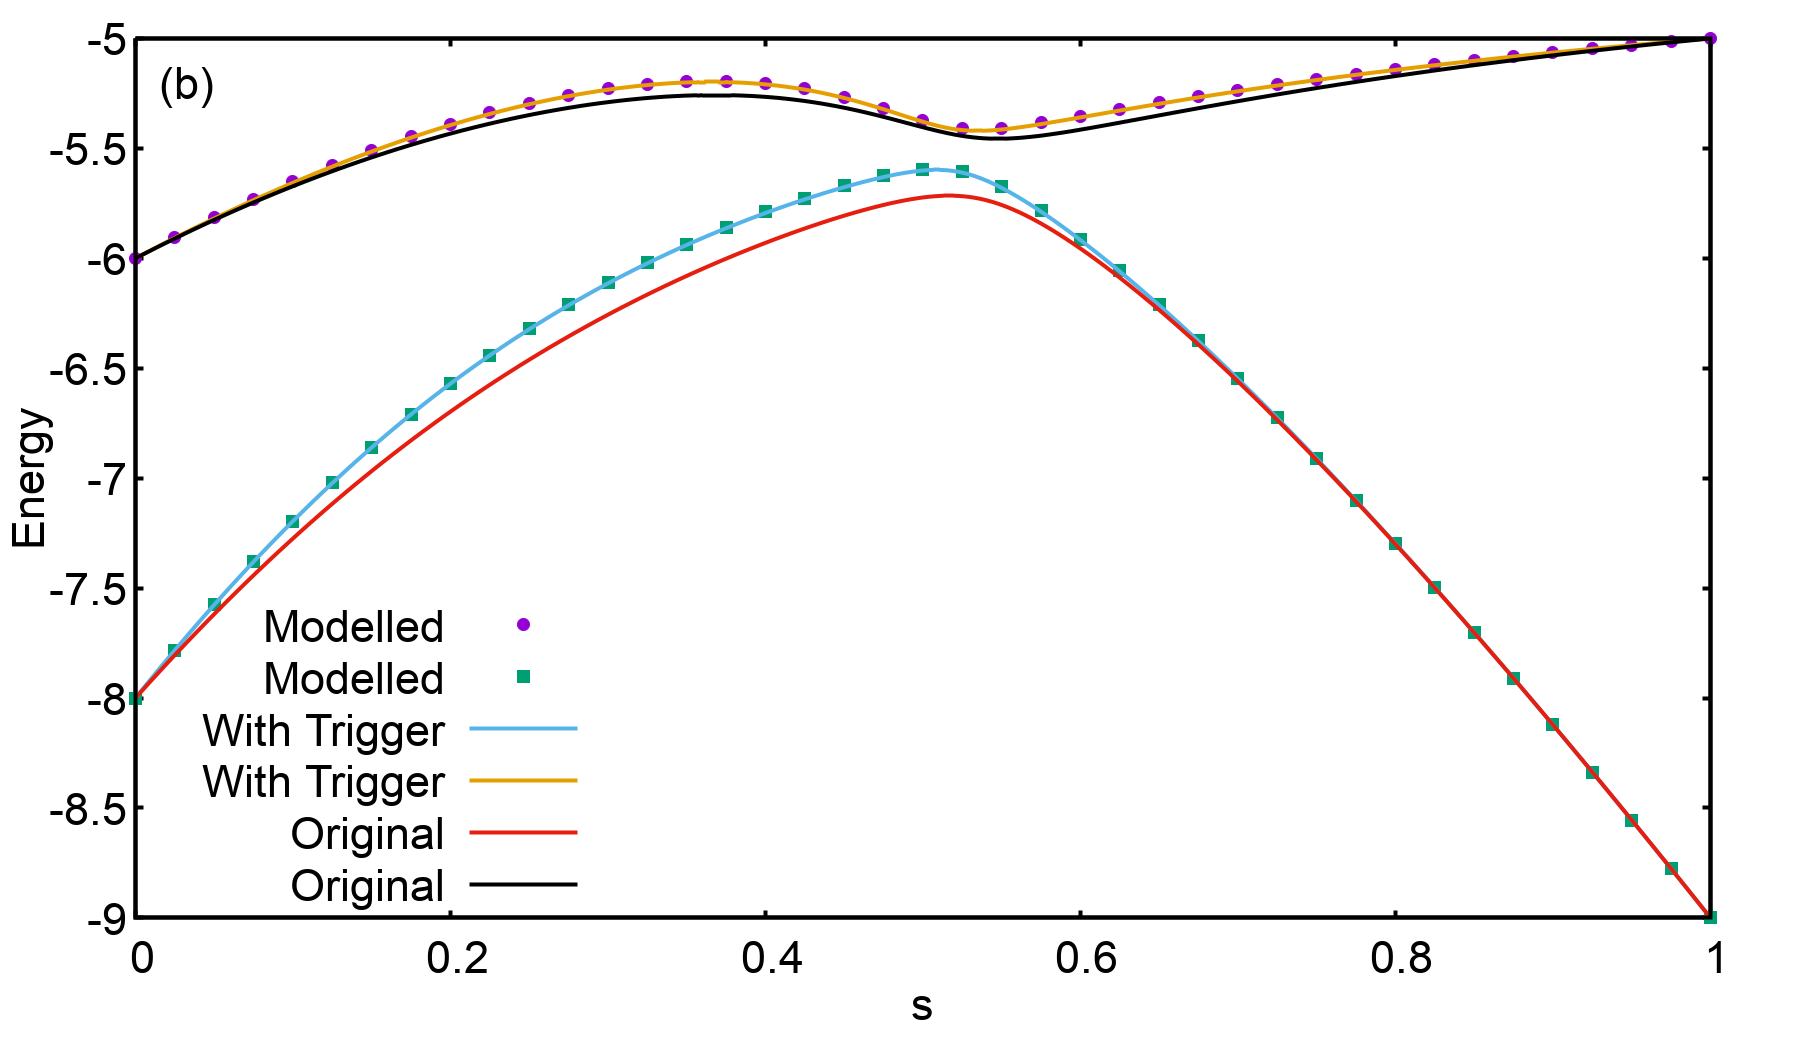
\includegraphics[scale=0.2]{59_antiFerro_g0.png}
\caption{The modelled energy levels after adding the triggers for $g$=0.1. (a): Ferromagnetic trigger; (b): Antiferromagnetic trigger. The energy levels obtained for the original Hamiltonian, and the Hamiltonian upon including the trigger Hamiltonian have also been shown.}
\label{fig:ap8}
\end{figure}
As can be observed from the figure, the effective Hamiltonian model can correctly describe the trend for the change in the minimum energy gap of the original Hamiltonian in both the cases. The energy levels of the Hamiltonian with stronger trigger Hamiltonians, cannot be modelled with only the two lowest lying energy states of the original Hamiltonian, and the higher energy states of the original Hamiltonian also need to be considered. Thus this simple approximation breaks down for higher $g$ values.
\section{Specific 12-spin problems}
Here, the energy spectra with the instantaneous energy expectation values of the state, and the overlap of the state of the system with the three lowest lying energy states of the instantaneous Hamiltonian are shown for some of the problems marked in the middle and bottom panel of Figure~(\ref{fig:a41}). These are:

\begin{itemize}
\item Problem 103, 319, and 705: The main reason for an improvement in the success probability in all of these problems is the proximity of the ground state and the first excited state for a longer time around one of the anti-crossings. The amplitude of the wavefunction of the state that transits to the first excited state at the first anti-crossing, oscillates between these two levels. This leads to a larger overlap of the final state with the ground state of the Hamiltonian. Shown here is the case for problem 103.
\begin{figure}
\centering 
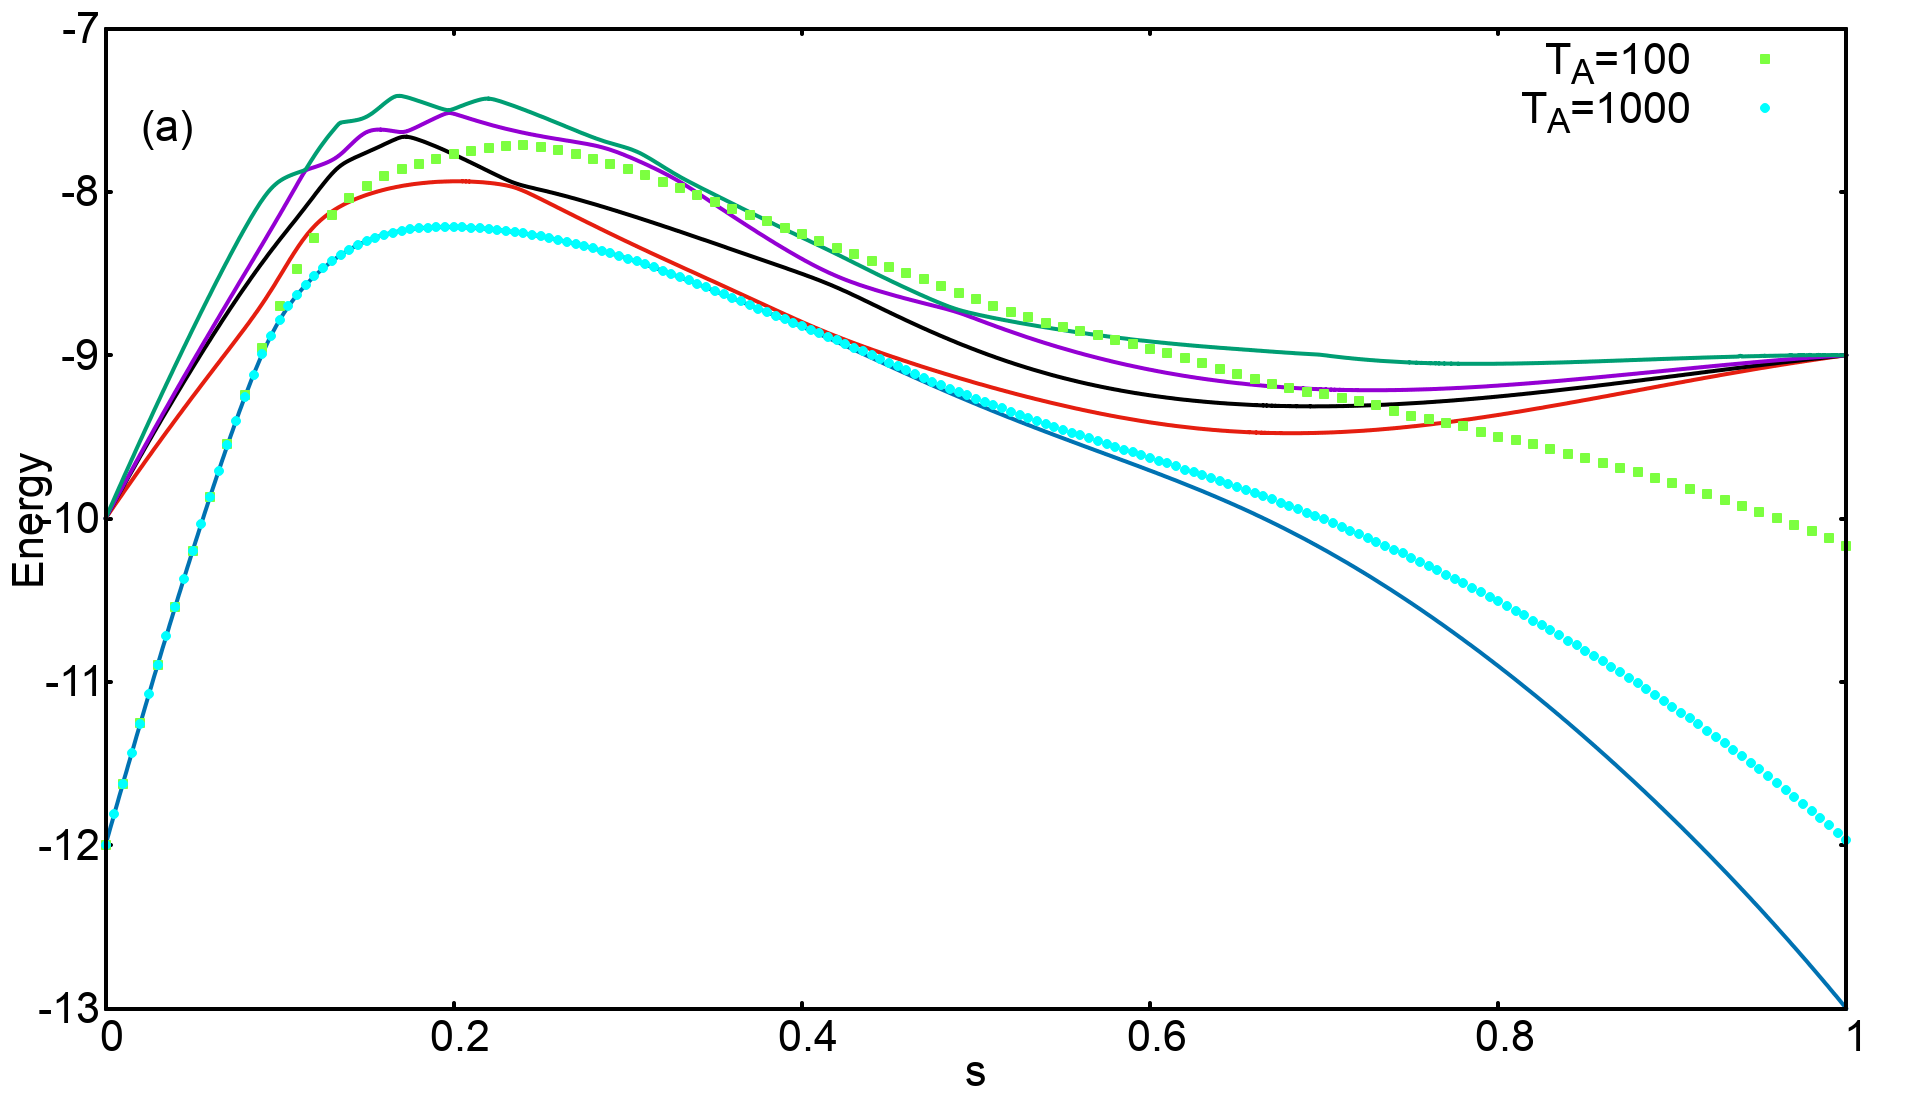
\includegraphics[scale=0.23]{103_A_g2.png}
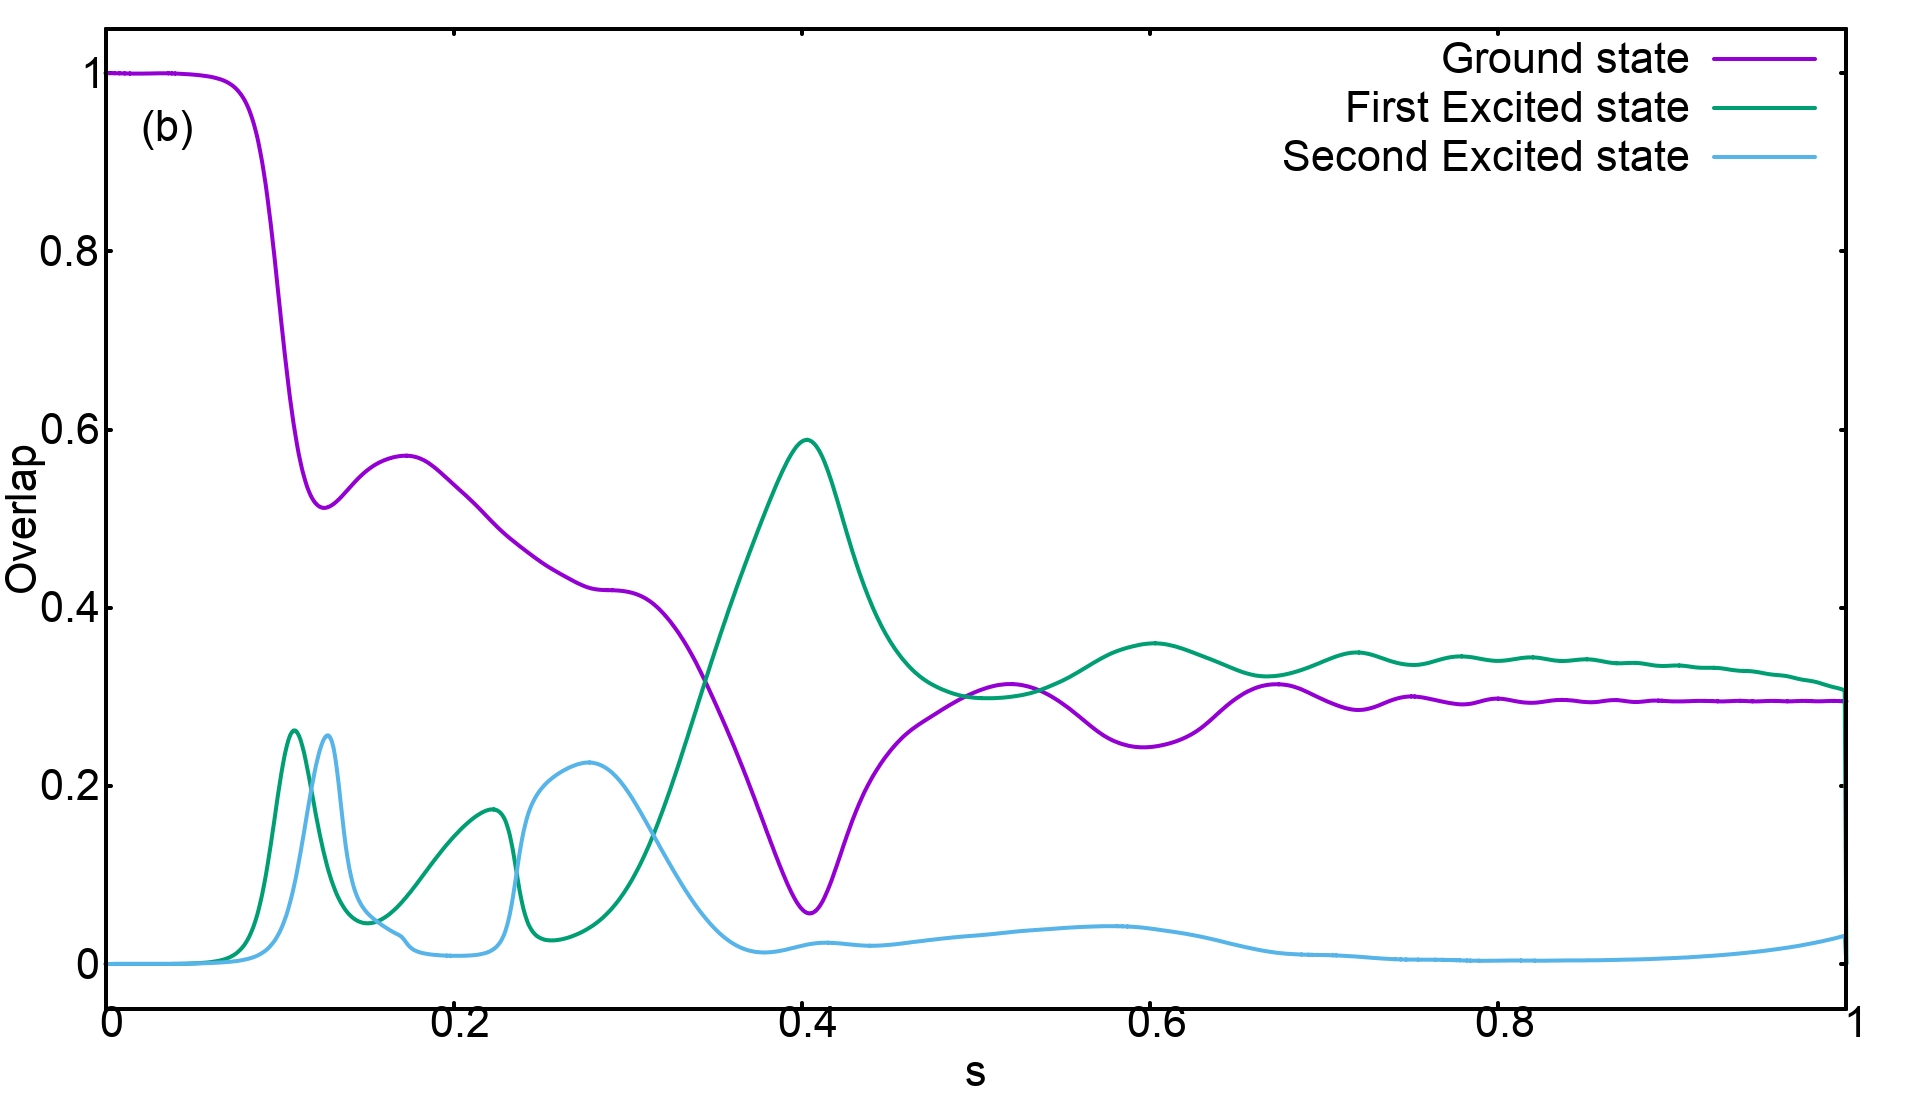
\includegraphics[scale=0.23]{103_A_g2_Overlap.png}
\caption{Problem 103: (a): The energy spectra and instantaneous energy expectation values corresponding to $T_A$=100, and $T_A$=1000; (b): The overlap of the system state with the three lowest lying energy levels of the instantaneous Hamiltonian for $T_A$=100.}
\label{fig:ap6}
\end{figure}

\item Problem 648 and 709: Both of these cases were found to have two anti-crossings (or crossings). The state of the system to shifts most of the amplitude to the first excited state at the first anti-crossing. Most of this amplitude then comes back to the ground state of the Hamiltonian at the second anti-crossing. This explains the improvement in the success probability. Shown here is the case for problem 709.
\begin{figure}
\centering 
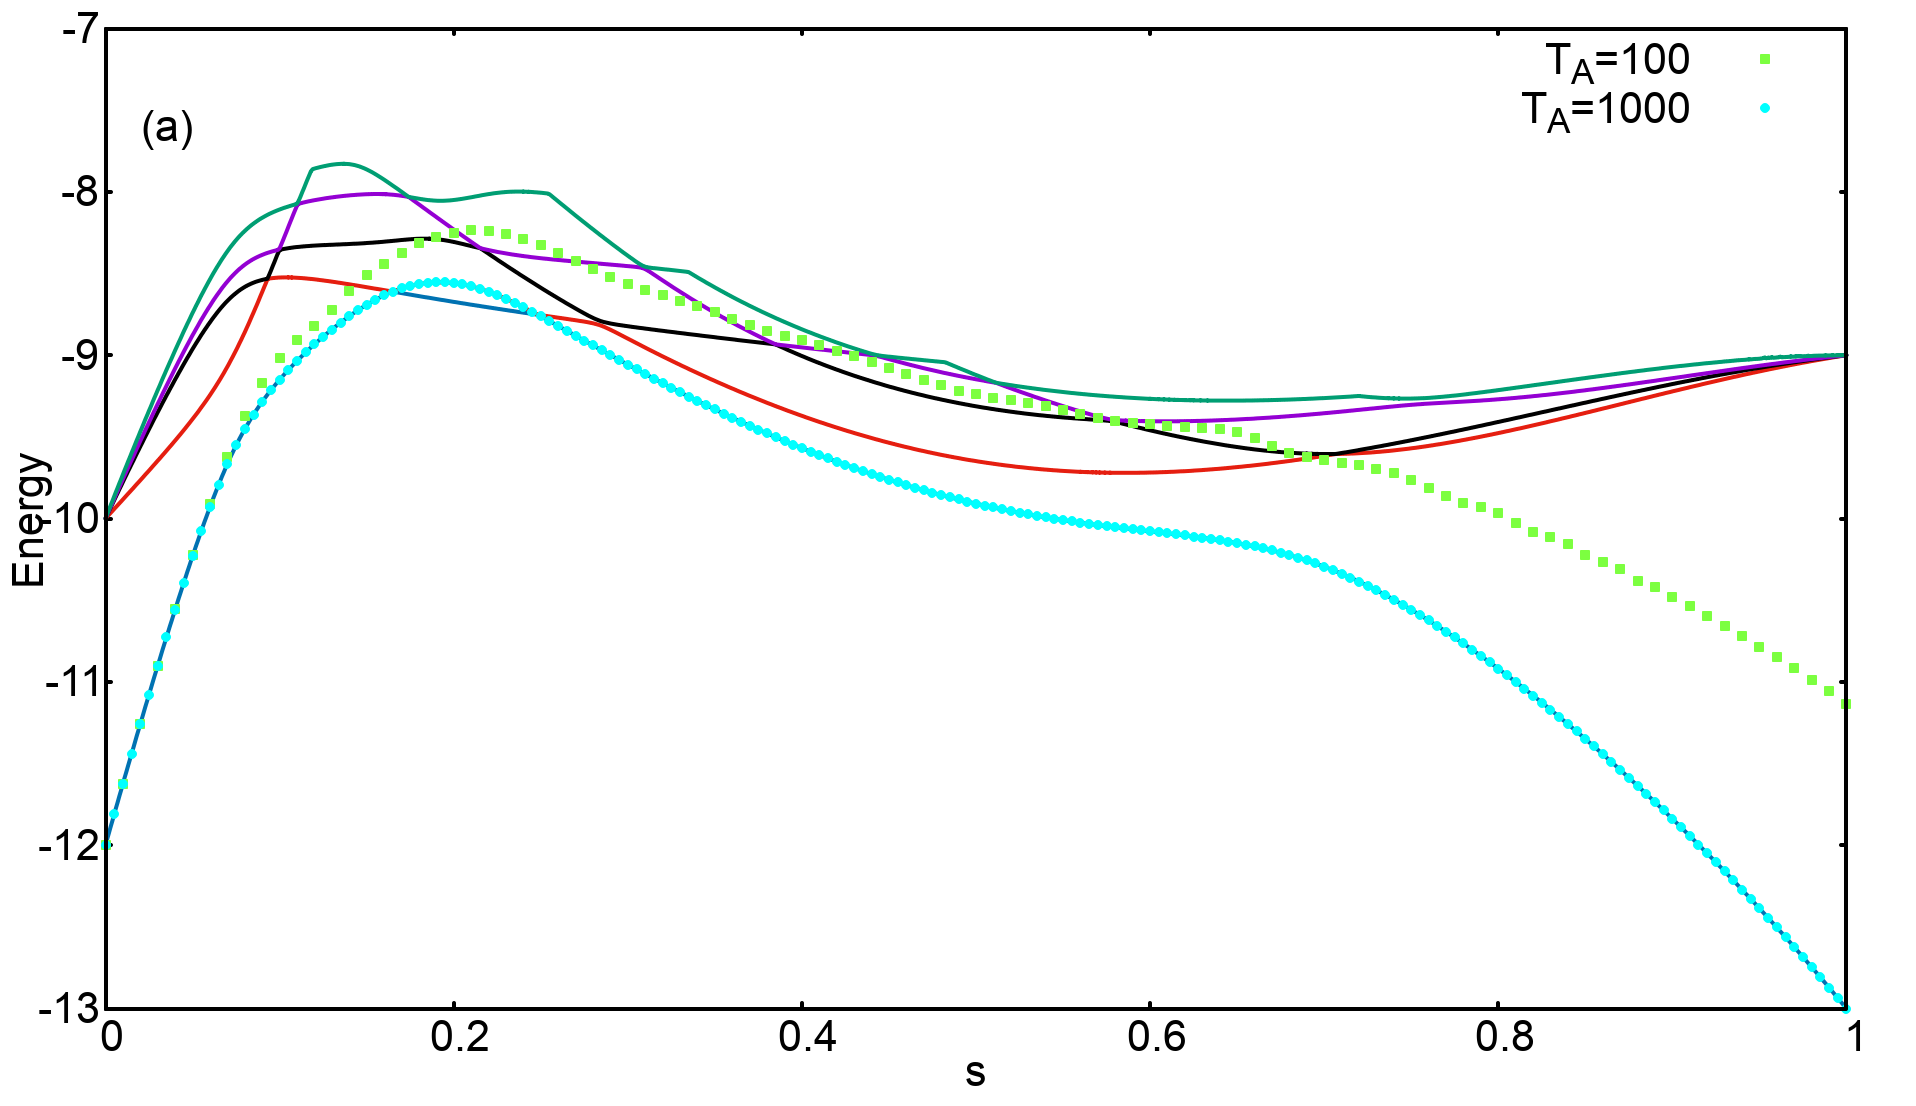
\includegraphics[scale=0.23]{709_A_g2.png}
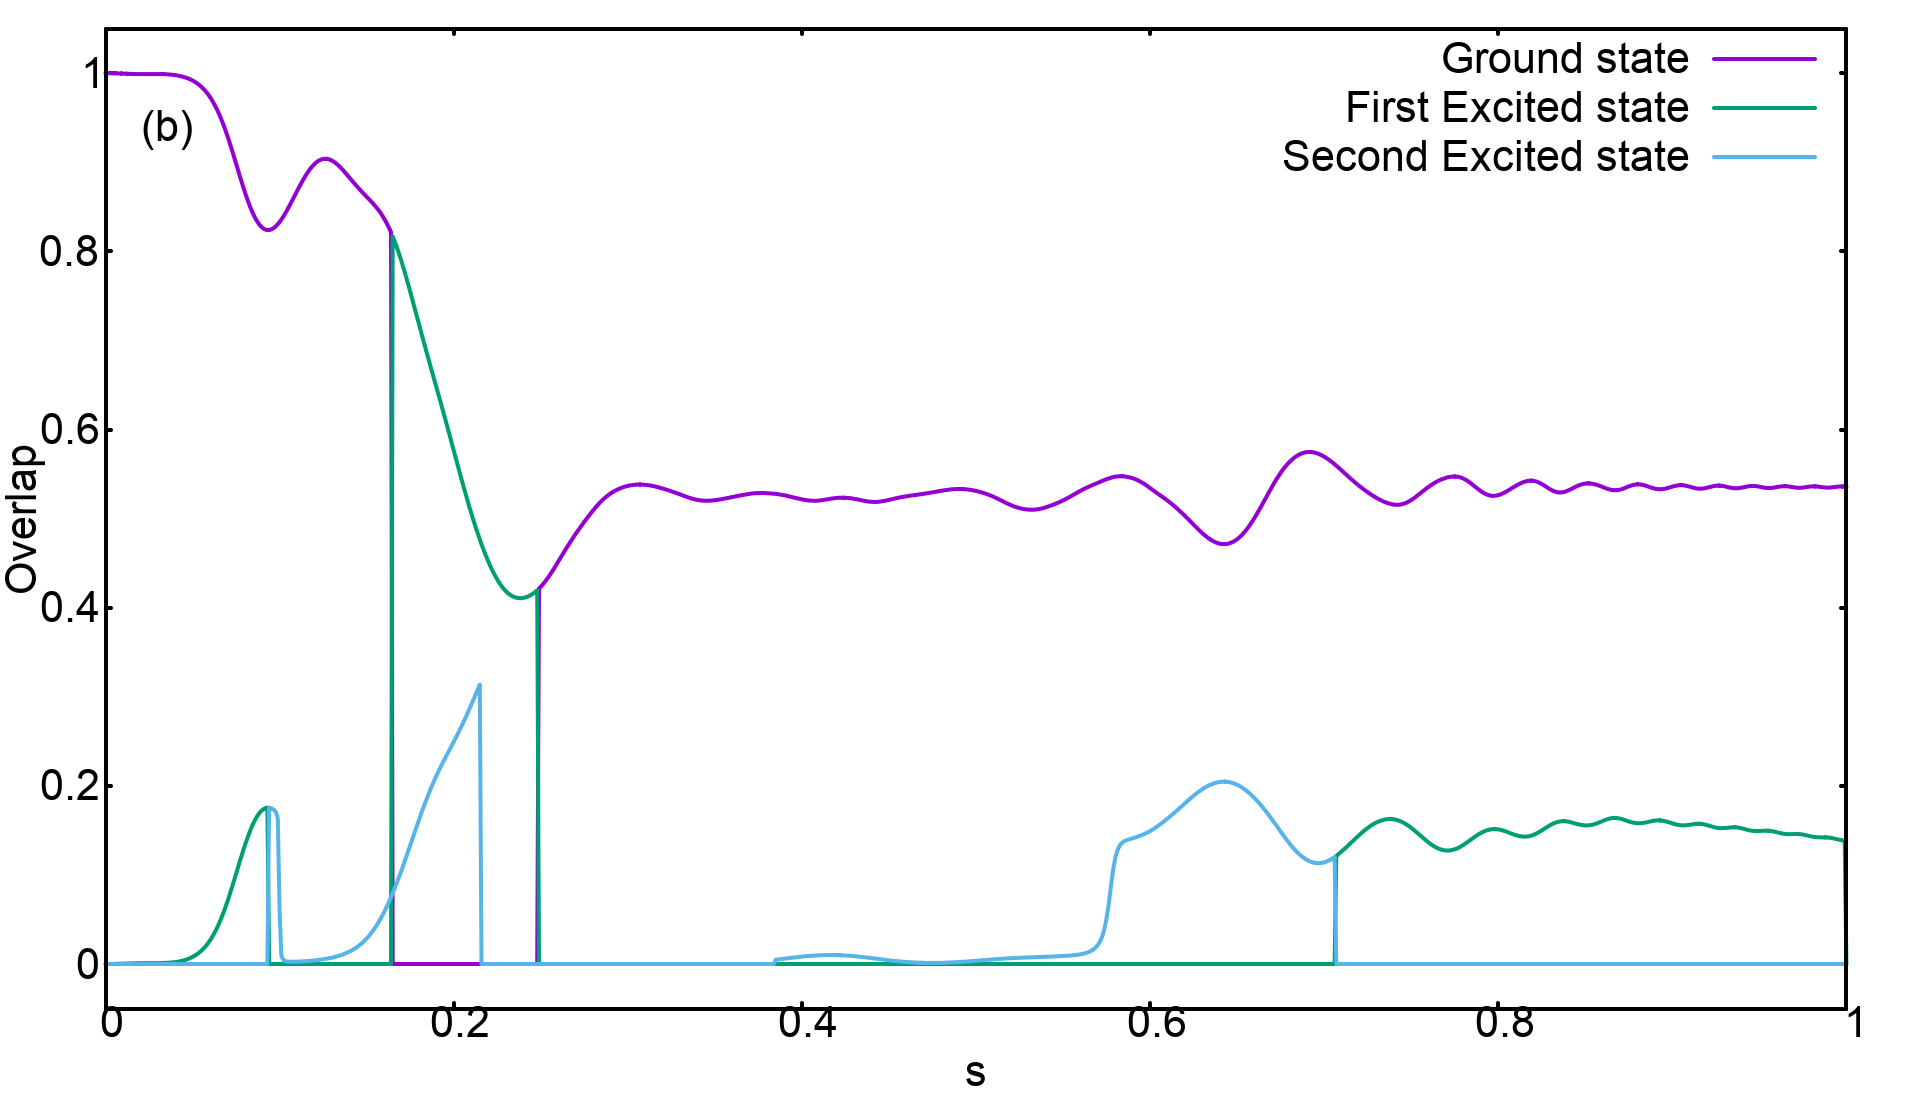
\includegraphics[scale=0.23]{709_A_g2_Overlap.png}
\caption{Problem 709: (a): The energy spectra and instantaneous energy expectation values corresponding to $T_A$=100, and $T_A$=1000; (b): The overlap of the system state with the three lowest lying energy levels of the instantaneous Hamiltonian for $T_A$=100.}
\label{fig:ap7}
\end{figure}
\end{itemize}
\end{appendices}
\end{document}
